\documentclass[a4paper, oneside,openany]{discothesis}

\usepackage[utf8]{inputenc}
\usepackage[T1]{fontenc}
\usepackage{anysize}
\marginsize{4cm}{2cm}{3cm}{3cm}
\usepackage{perpage} %the perpage package
\MakePerPage{footnote} %footnote counting per page

%additional packages
\usepackage{graphicx}
\usepackage{physics}
\usepackage{float}
\usepackage{bm}
\usepackage{siunitx}
\usepackage{multicol}
%%%%%%%%%%%%%%%%%%%%%%%%%%%%%%%%%%%%%%%%%%%%%%%%%%%%%%%%%%%%%%%%%%%%%%%%%%%%%%%%%%%%%%%%%%%%%%%%%
% DOCUMENT METADATA

\thesistype{PROPUESTA DE TESIS PARA OPTAR AL TÍTULO DE FÍSICO} % Master's Thesis, Bachelor's Thesis, Semester Thesis, Group Project
\title{ESTRUCTURA ESTELAR DE OBJETOS COMPACTOS CON UNA ECUACIÓN DE ESTADO NUMÉRICA}

\author{DAVID LEONARDO RAMOS SALAMANCA}
\email{}%david.ramos.salamanca@outlook.com}

\institute{%Grupo de Investigación en Relatividad y Gravitación  \\[2pt]
ESCUELA DE FÍSICA \\[2pt]
FACULTAD DE CIENCIAS \\[2pt]
UNIVERSIDAD INDUSTRIAL DE SANTANDER \\[2pt]
BUCARAMANGA \\[2pt]
2018}

% Optionally, you can put in your own logo here
%\logo{
\includegraphics[width=0.4\columnwidth]{figures/uislogo}}

\supervisors{LUIS A. NÚÑEZ DE VILLAVICENCIO MARTÍNEZ}
%\cosupervisors{}


% Optionally, titleabs, authorabs, keywords and categories of the work can be shown (on the Abstract page)
\keywords{Estructura estelar, ecuación de estado numérica}
\titleabs{Estructura estelar de objetos compactos con una ecuación de estado numérica\footnote{Propuesta de trabajo de grado}} %Title for abstract
\authorabs{David Leonardo Ramos Salamanca\footnote{Facultad de Ciencias. Escuela de física. Director: Luis A. Núñez de Villavicencio Martínez}} %Author for abstract
%\categories{ACM categories go here.}

%Información para abstract en otro idioma----------------------- 
\keywordss{Stellar structure, numerical equation of state}
\titleabss{Stellar structure of compact objects with a numerical equation of state\footnote{Bachellor thesis}} %Title for abstract
\authorabss{David Leonardo Ramos Salamanca\footnote{Facultad de Ciencias. Escuela de física. Adviser: Luis A. Núñez de Villavicencio Martínez}}

\date{\today}

%%%%%%%%%%%%%%%%%%%%%%%%%%%%%%%%%%%%%%%%%%%%%%%%%%%%%%%%%%%%%%%%%%%%%%%%%%%%%%%%%%%%%%%%%%%%%%%%%

\begin{document}

\frontmatter % do not remove this line
\maketitle

\cleardoublepage

%\begin{acknowledgements}
%	I thank Lorem ipsum dolor sit amet, consetetur sadipscing elitr, sed diam nonumy eirmod tempor invidunt ut labore et dolore magna aliquyam erat, sed diam voluptua. At vero eos et accusam et justo duo dolores et ea rebum. Stet clita kasd gubergren, no sea takimata sanctus est Lorem ipsum dolor sit amet. Lorem ipsum dolor sit amet, consetetur sadipscing elitr, sed diam nonumy eirmod tempor invidunt ut labore et dolore magna aliquyam erat, sed diam voluptua. At vero eos et accusam et justo duo dolores et ea rebum. Stet clita kasd gubergren, no sea takimata sanctus est Lorem ipsum dolor sit amet.
%\end{acknowledgements}


\begin{abstract}
    The abstract should be short, stating what you did and what the most important result is.
	Lorem ipsum dolor sit amet, consetetur sadipscing elitr, sed diam nonumy eirmod tempor invidunt ut labore et dolore magna aliquyam erat, sed diam voluptua. At vero eos et accusam et justo duo dolores et ea rebum. Stet clita kasd gubergren, no sea takimata sanctus est Lorem ipsum dolor sit amet. Lorem ipsum dolor sit amet, consetetur sadipscing elitr, sed diam nonumy eirmod tempor invidunt ut labore et dolore magna aliquyam erat, sed diam voluptua. At vero eos et accusam et justo duo dolores et ea rebum. Stet clita kasd gubergren, no sea takimata sanctus est Lorem ipsum dolor sit amet.\REMARK{¿Es necesario un abstract en la propuesta?}
\end{abstract}

%\begin{abstract1}
 %   The abstract should be short, stating what you did and what the most important result is.
%	Lorem ipsum dolor sit amet, consetetur sadipscing elitr, sed diam nonumy eirmod tempor invidunt ut labore et dolore magna aliquyam erat, sed diam voluptua. At vero eos et accusam et justo duo dolores et ea rebum. Stet clita kasd gubergren, no sea takimata sanctus est Lorem ipsum dolor sit amet. Lorem ipsum dolor sit amet, consetetur sadipscing elitr, sed diam nonumy eirmod tempor invidunt ut labore et dolore magna aliquyam erat, sed diam voluptua. At vero eos et accusam et justo duo dolores et ea rebum. Stet clita kasd gubergren, no sea takimata sanctus est Lorem ipsum dolor sit amet.
%\end{abstract1}



\tableofcontents

\mainmatter % do not remove this line

% Start writing here-------------------------------------------

\chapter{Introducción}

Los objetos compactos (también llamados estrellas compactas) son el residuo de la vida luminosa de las estrellas, llamados así porque su tamaño es significativamente más pequeño que el de una estrella normal/en la secuencia principal con una masa similar, estos objetos pueden alcanzar densidades superiores a la densidad de saturación nuclear  ($\rho_0=\num{2.3e+14}\,\si{g/cm^3}$) y a las que los potenciales gravitacionales son tan grandes que la relatividad general es importante para determinar su estructura (exceptuando a las enanas blancas). \REMARK{Quizá sea bueno introducir la clasificación de una}

Como remanentes de estrellas, vale la pena discutir a grandes rasgos el proceso de formación y evolución estelar antes de estudiar a mayor profundidad la estructura de los objetos compactos, ya que permitirá tener una idea general de los procesos que llevan a una estrella a su destino final.   \TODO{Pulir justificación} 

\section{Resumen de evolución estelar}
Las estrellas son formadas a partir de nubes de gas interestelar, compuestas en su mayoría de hidrógeno molecular, que debido a algún tipo de perturbación (como una onda de choque) comienzan a colapsar sobre ellas mismas gravitacionalmente. La energía gravitacional es convertida en calor por la contracción y si la temperatura incrementa lo suficiente ($T \approx 10^7 \, \si{\kelvin}$, punto de ignición para la fusión de hidrógeno a helio), con ayuda de la contracción adicional causada por la pérdida de energía por radiación, la fusión se convierte en la fuente de energía principal y la presión termal y de radiación balancearán la gravedad, permitiendo así que la estrella se forme \cite{Glendenning2000CompactStars}.

Las reacciones nucleares pueden sostener la estrella por un gran periodo de tiempo (de millones a billones de años, dependiendo de la masa de la estrella) en lo que se conoce como su fase de secuencia principal, llamada así porque las estrellas en esta etapa forman una secuencia mono-paramétrica (ignorando la composición química), cuyo parámetro es la masa estelar, en el diagrama de Hertzsprung-Russell (ver Figura \ref{HR}).
Las estrellas pasan la mayor parte de su vida luminosa en este estado, razón por la cual la mayoría de estrellas son encontradas en la secuencia principal, hasta que después de un tiempo característico el hidrógeno es extinguido/consumido/usado casi en su totalidad dejando un núcleo de Helio y da inicio a una siguiente etapa de fusión, de Helio a Carbono, el proceso se repite a lo largo de varias etapas de combustión (carbono, neón, oxígeno, magnesio y silicio) \cite{Scilla2016IntroductionEvolution}. \TODO{Revisar el orden del ciclo y por qué algunos elementos se saltan}

\begin{figure}[H]
    \centering
    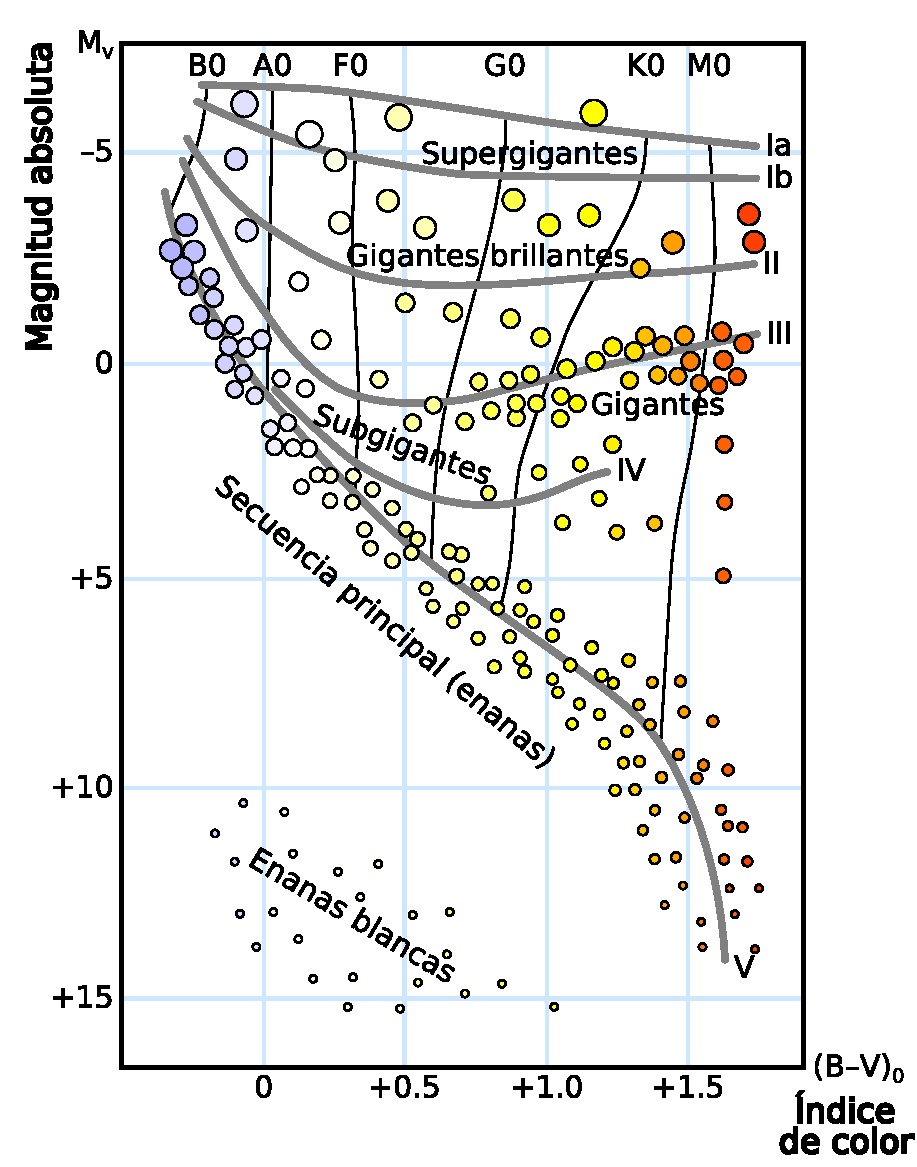
\includegraphics[width=250pt]{figures/H-R_diagram.pdf}%
    \caption{Diagrama Hertzsprung-Russell}
    \label{HR}
\end{figure}

%\begin{multicols}{2}[\columnsep2em] 

%\columnbreak
%\end{multicols}  
%y resultarán, después de un evento complejo y violento, como una estrella de neutrones o un agujero negro. \REMARK{No he hablado ni de estrellas de neutrones ni de agujeros negros...} 


El ciclo de combustión termina al alcanzar el hierro, debido a que la energía de enlace por nucleón tiene su valor máximo para el hierro y la fusión deja de ser exotérmica. Qué tanto avanza una estrella en este ciclo dependerá de la masa estelar, sólo estrellas masivas ($M \geq 8 M_{\odot} $) llegan al hierro/final, en este punto tendrán una estructura en forma de cascarones de materia que rodean al núcleo de hierro. Sin la energía producida por la fusión nuclear la compresión de la gravedad no tiene qué la equipare y la estrella colapsa, las capas de materia caen casi libremente hacia el núcleo desencadenando, a través de mecanismos complejos y no enteramente comprendidos, una supernova de colapso de núcleo \cite{Woosley2005TheSupernovae} \cite{Janka2012ExplosionSupernovae}.

El núcleo colapsado o proto-objeto compacto inicia un proceso de enfriamiento y reajustamiento estructural hasta que alcanza su composición de equilibrio de neutrones, protones, hiperones, leptones y posiblemente quarks, altamente degenerados, es decir, en un estado tal que han ocupado los niveles de energía más bajos disponibles. El objeto compacto formado será sostenido por la presión de degeneración de las partículas degeneradas que lo compongan \cite{Glendenning2000CompactStars}. Vale la pena aclarar que se acostumbra llamar a todos estos objetos estrellas de neutrones, aunque su composición puede ser tan variada como se mencionó antes.     
\TODO{Ya que se sabe qué es un objeto compacto, hablar a grandes rasgos de la estructura global de estos y la dependencia de la ecuación de estado, para darle paso a mi problema.}
\TODO{Papers seminales en estructura global y algunos de ecuaciones de estado.}

\chapter{Marco teórico}

\section{Estructura global de un objeto compacto}

\begin{equation}
\fdv{g}    
\end{equation}


\section{Estructura interna de objetos compactos y ecuaciones de estado}

\begin{figure}[H]
    \centering
    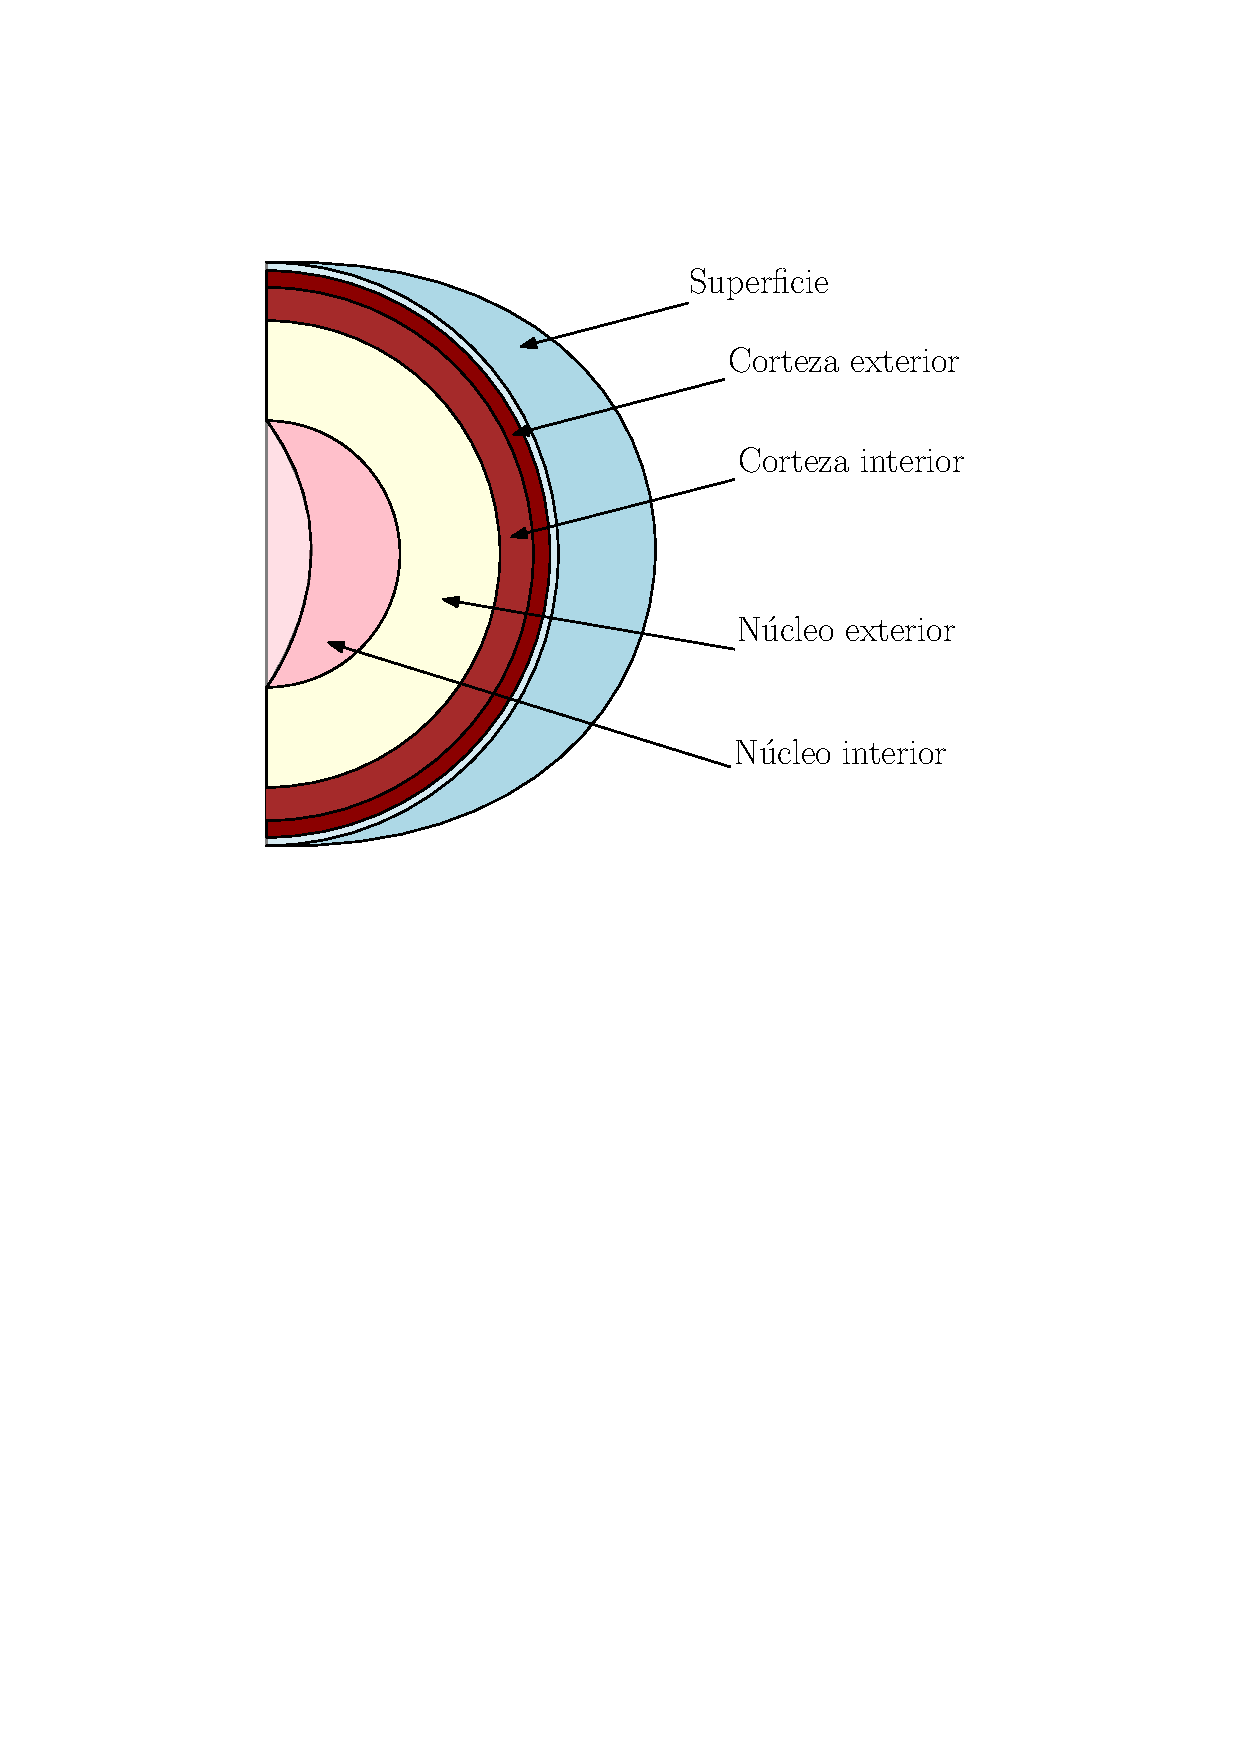
\includegraphics[width=200pt]{figures/neutronstar.pdf}
    \caption{Estructura interna de una estrella de neutrones}
    \label{NSS}
\end{figure}

\section{Criterios de estabilidad}

\chapter{Planteamiento del problema}
De los modelos estáticos surgen las primeras aproximaciones al estudio dinámico de objetos compactos: los efectos de la rotación lenta se pueden introducir mediante teoría de perturbaciones \cite{Hartle1967} y la evolución térmica se puede estudiar en un régimen cuasi-estático \cite{Becerra2013Quasi-staticObjects}. Es por esto que obtener soluciones a las ecuaciones de estructura relativistas, dada una determinada ecuación de estado para la materia densa, y verificar que los modelos obtenidos cumplan las condiciones de aceptabilidad física es muy importante a la hora de desarrollar modelos dinámicos de objetos compactos.

En este trabajo de grado se propone determinar si los modelos de estrellas de neutrones obtenidos a partir de las ecuaciones de estado más relevantes encontradas en la literatura son estables ante movimientos convectivos, usando la condición C11 propuesta por Nuñez et al.

\chapter{Objetivos}
\section{Objetivo general}
Determinar si los modelos de estrellas de neutrones obtenidos con las ecuaciones de estado encontradas en la literatura son estables ante convección.
\section{Objetivos específicos}
\begin{enumerate}
    \item Obtener modelos de estrellas de neutrones en equilibrio para las distintas ecuaciones de estado.
    \item Descartar los modelos que no cumplan las condiciones C1-C10.
    \item Evaluar a los modelos restantes ante convección adiabática usando el criterio C11.
\end{enumerate}
\chapter{Metodología}
\setcounter{footnote}{0}
Es importante resaltar que debido a que ecuaciones de TOV no se pueden resolver analíticamente y las ecuaciones de estado se encuentran tabuladas, la naturaleza del problema es computacional. 
Se propone como metodología para cumplir con los objetivos específicos planteados anteriormente cumplir las siguienets actividades:

\begin{enumerate}
    \item Reunir ecuaciones de estado para la materia densa tabuladas de la literatura, necesarias para resolver las ecuaciones de TOV.
    \item Interpolar las ecuaciones de estado manera óptima, explorando las distintas posibilidades.
    \item Resolver las ecuaciones de TOV numéricamente usando una ecuación de estado interpolada, para obtener modelos de estrellas de neutrones estáticas. Se usará en lo posible el ecosistema de software de código abierto para cómputo científico (SciPy\footnote{\url{https://www.scipy.org}}) de Python.
    \item Obtener las derivadas $\dv{P}{\rho}$ ,  $\dv{P}{r}$, $\dv[2]{P}{r}$, $\dv{\rho}{r}$ y $\dv[2]{\rho}{r}$, numéricamente. Esto permitirá evaluar la mayoría las condiciones de aceptabilidad física. 
    \item Variar la densidad central $\rho_c$ en las condiciones iniciales para obtener la familia de configuraciones en equilibrio asociada a la ecuación de estado y graficar las relaciones $M$-$R$ y $M$-$\rho_c$. Usado estos diagramas se puede identificar la masa máxima de la familia de soluciones y evaluar la condición C10, respectivamente.
\end{enumerate}
\section{Cronograma}
\definecolor{royalazure}{rgb}{0.0, 0.22, 0.66}
\centering
\vspace{-0.5cm}
\noindent\resizebox{0.28\textwidth}{!}{
\begin{ganttchart}[
    canvas/.append style={line width=.60pt,dotted},
    hgrid style/.style={line width=.60pt,dotted},
    vgrid={*1{ line width=.60pt,dotted}},
    title/.style={draw=none, fill=none},
    title label font=\bfseries\footnotesize,
    title label node/.append style={below=7pt},
    include title in canvas=false,
    group label font=\small\color{black},
    bar/.append style={fill=royalazure},
    group left shift=0,
    group right shift=0,
    bar height=.3,
    group peaks tip position=0,
    bar label node/.append style={left=0.6cm}
  ]{1}{4}
  \gantttitle[
    title label node/.append style={below left=7pt and -7pt}
  ]{\quad Mes:\quad 1}{1}
  \gantttitlelist{2,...,4}{1} \\ 
  \ganttbar{Actividad 1}{1}{1} \\[grid]
  \ganttbar{Actividad 2}{1}{2} \\[grid]
  \ganttbar{Actividad 3}{2}{3} \\[grid]
  \ganttbar{Actividad 4}{3}{4} \\[grid]
  \ganttbar{Actividad 5}{3}{4}
\end{ganttchart}}
\vspace{8cm}







% This displays the bibliography for all cited external documents. All references have to be defined in the file references.bib and can then be cited from within this document.
\bibliographystyle{IEEEtran}

\bibliography{references.bib}\TODO{Chequear que los links generados por Mendeley funcionen}

% This creates an appendix chapter, comment if not needed.
\appendix

%\chapter{Mi apéndice}

\end{document}